\section{Vokselių vizualizavimo ir normavimo įrankis}

Šiame skyriuje pristatomas šio darbo autoriaus sukurtas vokselių vizualizavimo
ir normavimo įrankis (Pav. \ref{fig:tool}), kuris remiasi tūriniu spindulių
skleidimu. Įrankis taip pat įgalina pasinaudoti transformavimo filtru ir šiame
darbe pasiūlytais globalaus permatomumo bei apšvietimo sustiprinimo filtrais.
Įrankis didžiąją dalį skaičiavimų atlieka GPU, o ne CPU.

\begin{figure}[!ht]
\centering
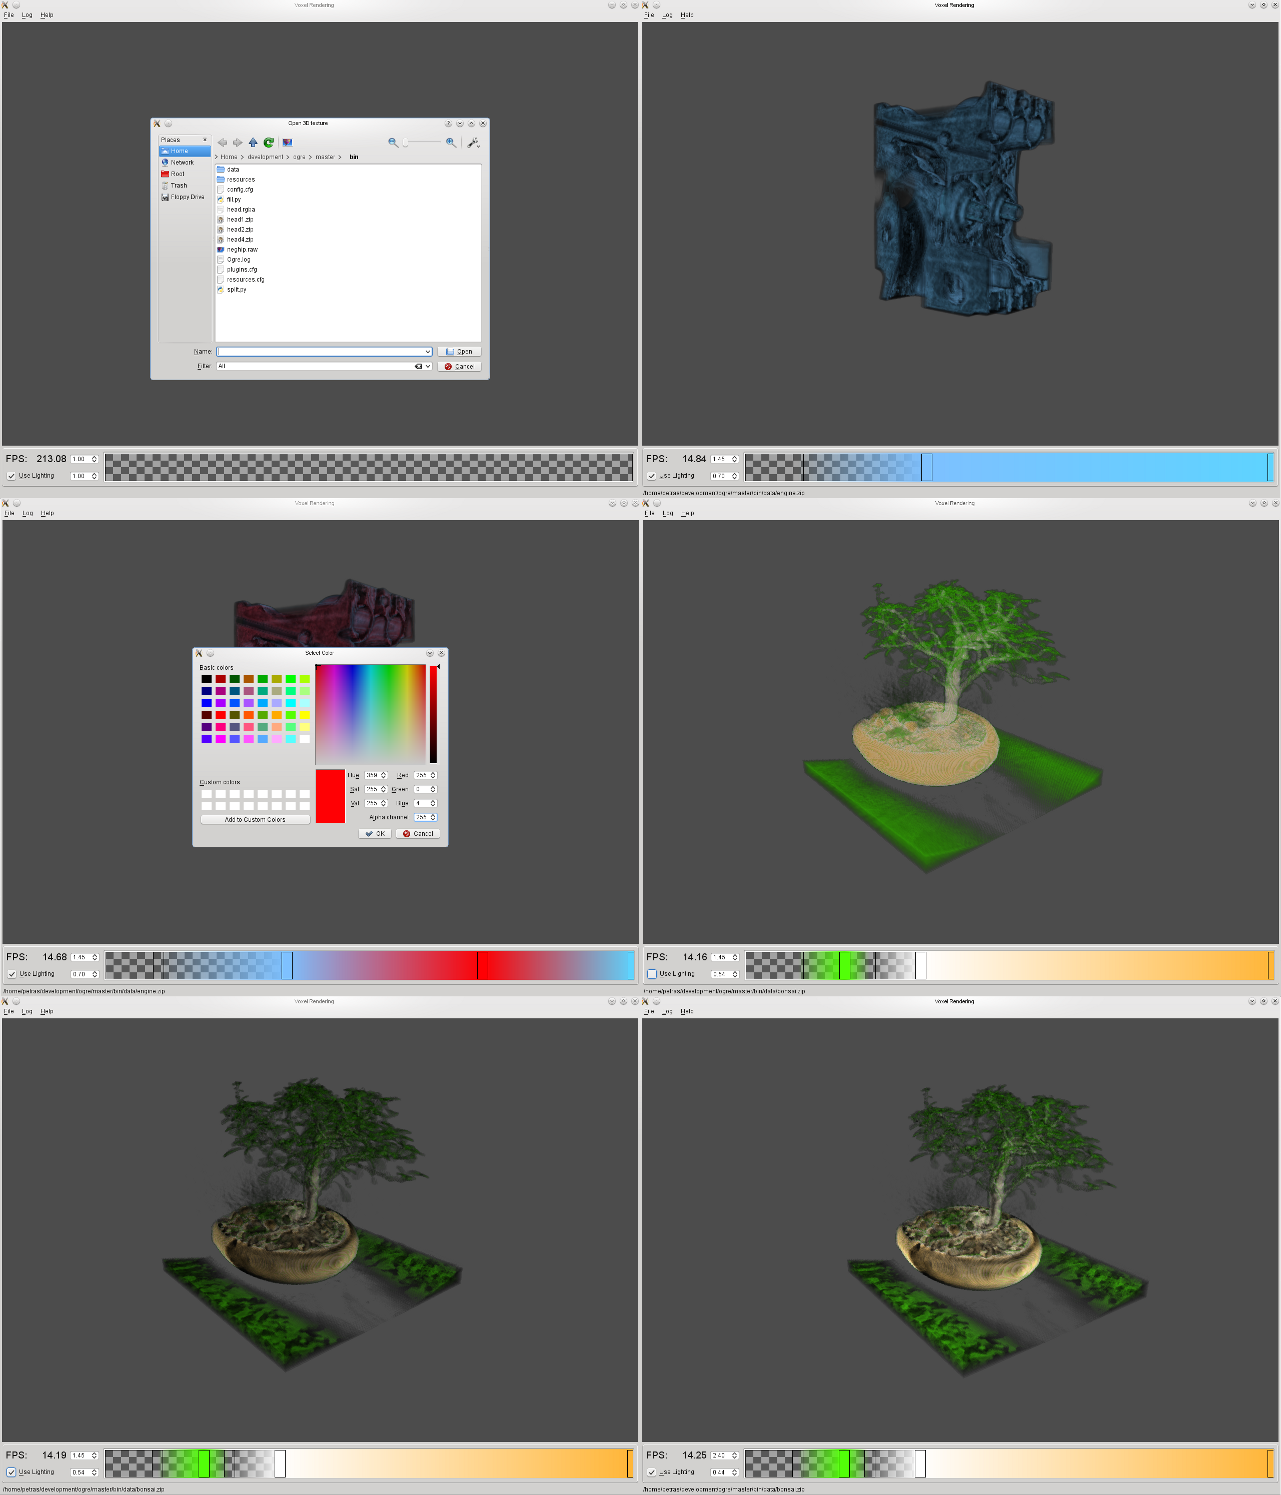
\includegraphics[height=15cm]{tool.png}
\caption{Vokselių vizualizavimo ir normavimo įrankis}
\label{fig:tool}
\end{figure}

